%%%%%%%%%%%%%%%%%%%%%%%%%%%%%%%%%%%%%%%%%%%%%%%%%%%%%%%%%%%%%%%%%%%%%%
% Lớp 11 | Hàm số lượng giác và phương trình lượng giác | Góc lượng giác
% Dạng 1D1?1-1: Câu hỏi lý thuyết
% Số câu: 39  (sinh tự động bởi tach_cau.py; từ nay thầy sửa trực tiếp file này)
%%%%%%%%%%%%%%%%%%%%%%%%%%%%%%%%%%%%%%%%%%%%%%%%%%%%%%%%%%%%%%%%%%%%%%

%%%%%%%%%%%%%%%% TRẮC NGHIỆM 4 PHƯƠNG ÁN %%%%%%%%%%%%%%%%

% nguồn: Ok_Toan11_TracNghiem_Lan2
\begin{ex}%[1D1N1-1]%[ma:0ae16de5]
	Quy ước chọn chiều dương của một đường tròn định hướng là 
	 \choice
		{Luôn cùng chiều quay kim đồng  hồ}
		{\True Luôn ngược chiều quay kim đồng  hồ}
		{Có  thể cùng chiều quay kim đồng hồ mà cũng có thể là ngược chiều quay kim đồng hồ}
		{Không cùng chiều quay kim  đồng hồ và cũng không ngược chiều quay kim đồng hồ}
	 \loigiai{
		Luôn ngược  chiều quay kim đồng hồ.
	} 
\end{ex}

% nguồn: Ok_Toan11_TracNghiem_Lan2
\begin{ex}%[1D1N1-1]%[ma:a1607c4f]
	Khẳng định nào sau đây là đúng khi nói về \lq\lq đường  tròn định hướng\rq\rq?
	 \choice
		{ Mỗi đường tròn  là một đường tròn định hướng}
		{ Mỗi đường tròn đã chọn một điểm là gốc đều là một  đường tròn định hướng}
		{ Mỗi đường tròn đã chọn một chiều chuyển động và một điểm là gốc đều là một  đường tròn định hướng}
		{\True Mỗi đường tròn trên đó ta đã chọn một chiều chuyển động gọi là chiều dương và chiều ngược lại được gọi là chiều âm là một đường tròn định hướng} 
	\loigiai{ 
		Mỗi đường tròn trên đó ta đã chọn một chiều chuyển động gọi là chiều dương và chiều  ngược lại được gọi là chiều âm là một đường tròn định hướng.
	 }
\end{ex}

% nguồn: Ok_Toan11_TracNghiem_Lan2
\begin{ex}%[1D1N1-1]%[ma:d2e834fa]
	Trên đường  tròn lượng giác gốc $A$ cho các góc lượng giác có số đo như sau:
	\begin{enumEX}[I.]{4}
		\item  $I$. $\dfrac{\pi}{4}$.
		\item  $II$. $-\dfrac{7\pi}{4}$.
		\item $III$. $\dfrac{13\pi}{4}$. 
		\item  $IV$. $-\dfrac{\sqrt{5}}{9}$.
	\end{enumEX}
	Hỏi  các góc lượng giác nào có điểm cuối trùng nhau?
	 \choice[2]
		{Chỉ  $I$ và $II$}
		{Chỉ  $I$, $II$ và $III$}
		 {Chỉ $II$, $III$ và $IV$}
		{\True Chỉ $I$, $II$ và  $IV$}
	\loigiai{ 
		 Ta có
		\begin{itemize}
			 \item $\dfrac{\pi}{4}-\left(-\dfrac{7\pi}{4} \right)=2\pi$ nên cung $I$ và $II$ trùng nhau.
			\item $\dfrac{\pi}{4}-\left(-\dfrac{71\pi}{4} \right)=18\pi=9\cdot2\pi$ nên cung $I$  và $IV$ trùng nhau.
		\end{itemize}
	 }
\end{ex}

% nguồn: Ok_Toan11_TracNghiem_Lan2
\begin{ex}%[1D1N1-1]%[ma:23cd3f1d]
	Trên đường tròn định hướng, mỗi cung lượng giác  $\wideparen{AB}$ xác định
	\choice 
		{  Một góc lượng giác tia đầu $OA$, tia cuối $OB$}
		{ Hai góc lượng giác tia  đầu $OA$, tia cuối $OB$}
		{ Bốn góc lượng  giác tia đầu $OA$, tia cuối $OB$}
		{\True Vô số góc lượng  giác tia đầu $OA$, tia cuối $OB$}
	\loigiai{ 
		Vô số góc lượng giác  tia đầu $OA$, tia cuối $OB$.
	 }
\end{ex}

% nguồn: Ok_Toan11_TracNghiem_Lan2
\begin{ex}%[1D1N1-1]%[ma:d34cbfa2]
	Trên đường tròn lượng giác với điểm gốc $A$. Có bao nhiêu điểm $N$ thỏa mãn $\left(OA, ON\right)=~30^\circ$? 
	 \choice
		{\True Có  duy nhất một điểm $N$}
		{Có hai  điểm $N$}
		{Có $4$ điểm $N$} 
		{Có vô  số điểm $N$}
	\loigiai{ 
		\begin{center}
			\begin{tikzpicture}[scale=1,font=\footnotesize,line join=round,line cap=round,>=stealth]
					 \def\r{2.5}
					 \draw[->] (-2.5,0)--(3,0) node[below]{$x$};
					\draw[->] (0,-2.5)--(0,2.5) node[right]{$y$}; 
					 \draw[fill=black] (0,0) node[below left]{$O$}
						 (30:2) circle (1pt) node[above right]{$M$}
						(2,0)  circle (1pt) node[above right]{$A$};
					 \draw (0:0.3*\r) arc (0:30:0.3*\r);
					\draw (0,0) circle (2); 
					\draw (0,0)--(30:2) 
						(15:0.45*\r) node{$30^\circ$}; 
				\end{tikzpicture}
		\end{center}
		Có  duy nhất một điểm $N$.
	} 
\end{ex}

% nguồn: Ok_Toan11_TracNghiem_Lan2
\begin{ex}%[1D1N1-1]%[ma:5f6a83d4]
	Khẳng định nào sau đây  là đúng khi nói về \lq\lq góc lượng giác\rq\rq?
	\choice 
		{  Trên đường tròn tâm $O$ bán kính $R=1$, góc hình học $AOB$ là góc lượng giác}
		{ Trên đường tròn tâm $O$ bán kính $R=1$, góc hình học $AOB$ có  phân biệt điểm đầu $A$ và điểm cuối $B$ là góc lượng giác}
		{ Trên đường tròn định hướng, góc hình học $AOB$ là góc lượng  giác}
		{\True Trên đường tròn định hướng, góc hình học  $AOB$ có phân biệt điểm đầu $A$ và điểm cuối $B$ là góc lượng giác}
	 \loigiai{
	Trên đường tròn định hướng, góc hình học $AOB$ có phân biệt điểm  đầu $A$ và điểm cuối $B$ là góc lượng giác.}
\end{ex}

% nguồn: Ok_Toan11_TracNghiem_Lan2
\begin{ex}%[1D1N1-1]%[ma:8e0d2575]
	Khẳng định nào sau đây là đúng khi  nói về \lq\lq đường tròn lượng giác\rq\rq?
	 \choice
		{ Mỗi đường tròn là một đường tròn lượng  giác}
		{ Mỗi đường tròn có  bán kính $R=1$ là một đường tròn lượng giác}
		{ Mỗi đường tròn có bán kính $R=1$, tâm trùng  với gốc tọa độ là một đường tròn lượng giác}
		{\True Mỗi đường tròn định hướng có bán kính $R=1$,  tâm trùng với gốc tọa độ là một đường tròn lượng giác}
	 \loigiai{
	Mỗi đường tròn định hướng có bán kính $R=1$, tâm trùng với gốc tọa độ  là một đường tròn lượng giác.}
\end{ex}

% nguồn: Ok_TracNghiemLop11_Lan1
\begin{ex}%[1D1N1-1]%[ma:c2a26e7a]
	Tìm mệnh đề  đúng.
	\choice 
		{$\pi$ rad  $=\left(\dfrac{180}{\pi} \right)$}
		{$\pi$  rad$=1^\circ$}
		 {$\pi$ rad $=60^\circ$}
		{\True $\pi$  rad $=180^\circ$}
	 \loigiai{
	} 
\end{ex}

% nguồn: Ok_TracNghiemLop11_Lan1
\begin{ex}%[1D1N1-1]%[ma:6a462cfe]
	Trên đường tròn lượng giác gốc $A$, biết góc lượng giác $(OA, OM)$ có số đo  bằng $420^\circ$, điểm $M$ nằm ở góc phần tư thứ mấy?
	\choice 
		{\True  $I$}
		{$III$} 
		{$II$} 
		{$IV$} 
	\loigiai{ 
	Ta có  sđ$(OA,OM)=420^\circ=60^\circ+360^\circ$. Vậy điểm $M$ nằm ở góc phần tư thứ $I$.}
\end{ex}

% nguồn: Ok_TracNghiemLop11_Lan1
\begin{ex}%[1D1N1-1]%[ma:4edcf2ce]
	Cho $\dfrac{\pi}{2}<a<\pi$. Kết quả  đúng là
	 \choice
		{$\sin a>0$,  $\cos a>0$}
		 {$\sin a<0$, $\cos a<0$}
		 {\True $\sin a>0$, $\cos a<0$}
		{$\sin a<0$, $\cos a>0$} 
	\loigiai{ 
		Vì $\dfrac{\pi}{2}<a<\pi$ nên $\sin a>0$,  $\cos a<0$.
	 }
\end{ex}

% nguồn: Ok_TracNghiemLop11_Lan1
\begin{ex}%[1D1N1-1]%[ma:8dd208c8]
	\immini[thm]{Trong mặt phẳng tọa độ $Oxy,$ trên đường tròn lượng giác như hình vẽ, cho góc lượng giác có tia đầu là  $OA$ và số đo là $135^\circ$. Hỏi tia cuối của góc lượng giác đã cho là tia nào dưới đây?
	 \choice
		{$OQ$} 
		 {$OP$}
		 {$OM$}
		{\True $ON$} 
		 }
		{\begin{tikzpicture}[scale=.7,>=stealth,font=\footnotesize,line join=round,line cap=round]
		\draw[fill](0,0) coordinate (O)  node[below left]{$O$} circle (1pt)
			(2,0) coordinate (A) node[below right]{$A$} circle (1.5  pt)
			(45:2) coordinate (M) node [above] {$M$} circle (1.5 pt) 
			(135:2) coordinate (N) node [above] {$N$} circle  (1pt)
			(225:2) coordinate (P) node [below left]  {$P$} circle (1pt)
			(-45:2)  coordinate (Q) node [below] {$Q$} circle (1pt);
		\draw (0,0) circle (2  cm);
		\draw[->] (-3,0)--(3,0) node [below]{$x$}; 
		\draw[->] (0,-3)--(0,3) node  [left]{$y$};
		\clip (-5,-5)  rectangle (5,5);
	\end{tikzpicture}
		} 
	\loigiai{ 
	Quan sát hình vẽ  ta thấy góc lượng giác $(OA,ON)=135^\circ$.}
\end{ex}

% nguồn: Ok_TracNghiemLop11_Lan1
\begin{ex}%[1D1N1-1]%[ma:0d6b1b1a]
	Trong các mệnh đề sau, mệnh đề nào  đúng ?
	\choice 
		{Các hàm số $y=\sin x$, $ y=\cos x$, $y=\cot x$  đều là hàm số chẵn}
		{\True Các hàm số $y=\sin x$, $y=\cot x$, $y=\tan  x$ đều là hàm số lẻ}
		 {Các hàm số $y=\sin x$, $y=\cos x$, $y=\tan x$ đều là hàm số chẵn}
		{Các hàm số $y=\sin x$, $y=\cos x$, $y=\cot x$ đều là hàm số lẻ} 
	\loigiai{ 
		 Hàm số $y=\sin x$, $y=\tan x$, $y=\cot x$ là hàm số lẻ.\\
	Hàm số $y=\cos x$ là hàm số  chẵn. }
\end{ex}

% nguồn: Ok_TracNghiemLop11_Lan1
\begin{ex}%[1D1N1-1]%[ma:9271d260]
	Cho góc có số đo $\alpha$ thuộc góc phần tư thứ nhất của đường tròn lượng giác.  Hãy chọn kết quả đúng trong các kết quả sau đây?
	 \choice
		 {$\cot\alpha<0$}
		{$\tan\alpha<0$} 
		{$\cos\alpha<0$} 
		{\True  $\sin\alpha>0$}
	 \loigiai{
		Góc có  số đo $\alpha$ thuộc góc phần tư thứ nhất nên $\heva{&\sin\alpha>0\\&\cos\alpha>0\\&\tan \alpha>0\\&\cot\alpha>0.}$
	} 
\end{ex}

% nguồn: Ok_Toan11_TracNghiem_Lan2
\begin{ex}%[1D1H1-1]%[ma:7799d634]
	Trên đường tròn lượng giác có điểm gốc là $A$. Điểm $M$ thuộc đường tròn sao cho cung lượng giác $AM$ có số đo $45^\circ$. Gọi  $N$ là điểm đối xứng với $M$ qua trục $Ox$, số đo cung lượng giác $AN$ bằng
	\choice 
		 {$-45^\circ$}
		 {$315^\circ$}
		 {$45^\circ$ hoặc $315^\circ$}
		{\True $-45^\circ + k360^\circ$,  $k \in \mathbb{Z}$}
	\loigiai{ 
		Vì số đo cung $AM$ bằng $45^\circ$ nên $\widehat{AOM} = 45^\circ$, $N$ là điểm đối  xứng với $M$ qua trục $Ox$ nên $\widehat{AON} = 45^\circ$.\\
		Do đó số  đo cung $AN$ bằng $45^\circ$ nên số đo cung lượng giác $AN$ có số đo là $-45^\circ + k360^\circ$, $k \in \mathbb{Z}$.
	} 
\end{ex}

% nguồn: Ok_Toan11_TracNghiem_Lan2
\begin{ex}%[1D1H1-1]%[ma:5ba92351]
	Trên đường tròn với điểm gốc là $A$. Điểm $M$ thuộc đường tròn sao cho cung lượng giác $AM$ có số đo $60^\circ$. Gọi $N$  là điểm đối xứng với điểm $M$ qua trục $Oy$, số đo cung $AN$ là
	 \choice
		 {\True $120^\circ$}
		{$-240^\circ$} 
		 {$-120^\circ$ hoặc $240^\circ$}
		{$120^\circ + k360^\circ$, $k \in  \mathbb{Z}$}
	 \loigiai{
	\immini 
		 {Ta có $\widehat{AOM} = 60^\circ$, $\widehat{MON} = 60^\circ$.\\
		 Nên $\widehat{AON} = 120^\circ$. Khi đó số đo cung $AN$ bằng $120^\circ$.
		 }
		{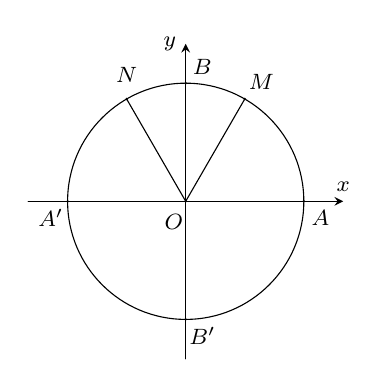
\begin{tikzpicture}[declare function={r=3;},line join = round,line cap = round,>=stealth,font=\footnotesize,scale=0.5]
		\tikzset{label style/.style={font=\footnotesize}} 
		\path (0,0) coordinate (O) 
			(3,0)  coordinate (A)
			(0,3)  coordinate (B)
			(0,-3) coordinate (B') 
			(-3,0)  coordinate (A')
			(0:0)++(60:3) coordinate (M) 
			(0:0)++(120:3) coordinate (N); 
		 \draw[->] (-4,0) -- (4,0) node[above]{$x$};
		\draw[->] (0,-4) -- (0.,4)  node[left]{$y$};
		\draw  (O) circle (r);
		\draw (N)--(O)--(M); 
		\pgfmathsetmacro{\R}{1.2*r} 
		\foreach  \p/\r in {A/-45,O/-120,A'/-135,B'/-45,B/45,M/45,N/90}
		\fill (\p) circle (1pt) node[shift={(\r:3mm)}]{$\p$}; 
	\end{tikzpicture}
		} 
	} 
\end{ex}

% nguồn: Ok_Toan11_TracNghiem_Lan2
\begin{ex}%[1D1H1-1]%[ma:48671dbf]
	Cho góc lượng giác $(Ox, Oy) = 22^\circ  30' + k360^\circ$. Với giá trị $k$ bằng bao nhiêu thì góc $(Ox, Oy) = 1822^\circ 30'$?
	\choice 
		 {$k \in \varnothing$}
		{$k  = 3$}
		 {$k = 4$}
		{\True $k  = 5$}
	 \loigiai{
		Theo đề $(Ox, Oy) = 1822^\circ 30' \Rightarrow 22^\circ 30' + k\cdot 360^\circ = 1822^\circ 30'  \Rightarrow k = 5$.
	 }
\end{ex}

% nguồn: Ok_Toan11_TracNghiem_Lan2
\begin{ex}%[1D1H1-1]%[ma:5079528b]
	Các cặp góc lượng giác sau ở trên cùng một đường tròn đơn vị, cùng tia đầu và tia cuối. Hãy nêu kết  quả \textbf{sai} trong các kết quả sau đây
	\choice 
		 {$\dfrac{\pi}{3}$ và $-\dfrac{35\pi}{3}$}
		 {\True $\dfrac{\pi }{10}$ và $\dfrac{152\pi}{5}$}
		{$-\dfrac{\pi}{3}$  và $\dfrac{155\pi}{3}$}
		{$\dfrac{\pi}{7}$ và  $\dfrac{281\pi}{7}$}
	\loigiai{ 
		Cặp góc lượng giác $a$ và $b$ ở trên cùng một đường tròn đơn vị, cùng tia  đầu và tia cuối.\\
		Khi đó $a = b + k2\pi$, $k \in \mathbb{Z}$ hay  $k = \dfrac{a - b}{2\pi}$.\\
		Với cặp $\dfrac{\pi }{10}$ và $\dfrac{152\pi}{5}$ ta có  $k = \dfrac{\dfrac{\pi }{10} - \dfrac{152\pi}{5}}{2\pi} = -\dfrac{-303}{20} \notin \mathbb{Z}$.\\
		Suy ra cặp $\dfrac{\pi }{10}$  và $\dfrac{152\pi}{5}$ không thỏa mãn.
	} 
\end{ex}

% nguồn: Ok_Toan11_TracNghiem_Lan2
\begin{ex}%[1D1H1-1]%[ma:e8e036cb]
	Trên đường tròn lượng  giác gốc $A$, cung lượng giác nào có các điểm biểu diễn tạo thành hình vuông?
	 \choice
		{\True $\dfrac{k\pi}{2}$, $k  \in \mathbb{Z}$}
		{ $ k\pi$,  $k \in \mathbb{Z}$}
		{ $\dfrac{k2\pi}{3}$, $k  \in \mathbb{Z}$}
		{ $\dfrac{k\pi}{3}$,  $k \in \mathbb{Z}$}
	\loigiai{ 
		Hình vuông $CDEF$ có góc $\widehat{DCE}$ là $45^\circ$ nên góc ở tâm là $90^\circ$ tương  ứng $\dfrac{k\pi}{2}$, $k \in \mathbb{Z}$.
	 }
\end{ex}

% nguồn: Ok_Toan11_TracNghiem_Lan2
\begin{ex}%[1D1H1-1]%[ma:a2a6d55c]
	Cho bốn cung (trên một đường tròn định hướng): $\alpha = -\dfrac{5\pi}{6}$, $\beta = \dfrac{\pi}{3}$, $\gamma =\dfrac{25\pi}{3}$, $\delta = \dfrac{19\pi }{6}$. Các cung nào có điểm cuối trùng nhau? 
	 \choice
		{$\alpha  $ và $\beta$; $\gamma$ và $\delta$}
		{\True $\beta $ và $\gamma$; $\alpha$ và  $\delta$}
		{  $\alpha$, $\beta$, $\gamma$}
		{$\beta$, $\gamma$, $\delta$} 
	\loigiai{ 
		\textbf{Cách 1:} Ta có $\delta -\alpha  = 4\pi \Rightarrow$ hai cung $\alpha$ và $\delta$ có điểm cuối trùng nhau.\\
		Và $\gamma -\beta = 8\pi \Rightarrow$  hai cung $\beta$ và $\gamma$ có điểm cuối trùng nhau.\\
		\textbf{Cách 2:} Gọi $A$, $B$, $C$, $D$ là điểm cuối của các cung $\alpha$, $\beta$,  $\gamma$, $\delta$.\\
		Biểu diễn các cung trên đường tròn lượng giác  ta có $B \equiv C$, $A \equiv D$.
	 }
\end{ex}

% nguồn: Ok_Toan11_TracNghiem_Lan2
\begin{ex}%[1D1H1-1]%[ma:2a15d4ce]
	Trên đường tròn lượng giác gốc  $A$, cung lượng giác nào có các điểm biểu diễn tạo thành tam giác đều?
	\choice 
		{\True $\dfrac{k2\pi}{3}$, $k \in \mathbb{Z}$} 
		{ $k\pi$, $k  \in \mathbb{Z}$}
		{ $\dfrac{k\pi}{2}$, $k  \in \mathbb{Z}$}
		{  $\dfrac{k\pi}{3}$, $k \in \mathbb{Z}$}
	 \loigiai{
	Tam giác đều có góc ở đỉnh là ${60^o}$ nên góc ở tâm là ${120^o}$ tương ứng  $\dfrac{k2\pi}{3}$, $k \in \mathbb{Z}$.}
\end{ex}

% nguồn: Ok_Toan11_TracNghiem_Lan2
\begin{ex}%[1D1H1-1]%[ma:8be52505]
	Một chiếc đồng hồ, có kim chỉ giờ $OG$ chỉ số $9$ và kim phút $OP$  chỉ số $12$. Số đo của góc lượng giác $(OG, OP)$ là
	 \choice
		{\True $\dfrac{\pi}{2} +  k2\pi$, $k \in \mathbb{Z}$}
		{$-270^\circ  + k360^\circ$, $k \in \mathbb{Z}$}
		{$270^\circ + k360^\circ$, $k \in  \mathbb{Z}$}
		{$\dfrac{9\pi}{10} + k2\pi$, $k \in \mathbb{Z}$} 
	 \loigiai{
		Góc lượng giác $(OG, OP)$ chiếm $\dfrac{1}{4}$  đường tròn.\\
		Số đo là  $\dfrac{1}{4} \cdot 2\pi + k2\pi$, $k \in \mathbb{Z}$.
	} 
\end{ex}

% nguồn: Ok_Toan11_TracNghiem_Lan2
\begin{ex}%[1D1H1-1]%[ma:437fe0c1]
	Trên  đường tròn lượng giác với điểm gốc là $A$. Điểm $M$ thuộc đường tròn sao cho cung lượng giác $AM$ có số đo $75^\circ$. Gọi $N$ là điểm đối xứng với điểm $M$ qua gốc tọa độ $O$, số đo cung lượng giác $AN$ bằng
	 \choice
		 {$255^\circ$}
		 {$-105^\circ$}
		{$-105^\circ$ hoặc  $255^\circ$}
		{\True $-105^\circ + k360^\circ$,  $k \in \mathbb{Z}$}
	\loigiai{ 
	 \immini
		{Ta có $\widehat{AOM} = 75^\circ$, $\widehat{MON}  = 180^\circ$.\\
		 Nên cung lượng giác $AN$ có số đo bằng $-105^\circ + k360^\circ$, $k \in \mathbb{Z}$.
		} 
		{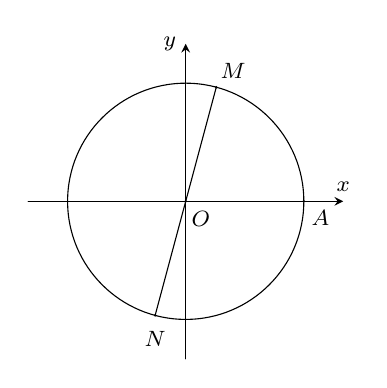
\begin{tikzpicture}[declare function={r=3;},line join = round,line cap = round,>=stealth,font=\footnotesize,scale=0.5]
		\tikzset{label style/.style={font=\footnotesize}} 
		\path (0,0)  coordinate (O)
			 (3,0) coordinate (A)
			(0,3)  coordinate (B)
			(0,-3) coordinate (B') 
			(-3,0) coordinate  (A')
			(0:0)++(75:3) coordinate (M) 
			(0:0)++(255:3)  coordinate (N);
		\draw[->] (-4,0) -- (4,0) node[above]{$x$}; 
		\draw[->] (0,-4) -- (0.,4)  node[left]{$y$};
		\draw  (O) circle (r);
		\draw  (N)--(O)--(M);
		 \pgfmathsetmacro{\R}{1.2*r}
		\foreach \p/\r in  {A/-45,O/-50,M/45,N/-90}
		 \fill (\p) circle (1pt) node[shift={(\r:3mm)}]{$\p$};
	\end{tikzpicture}
		 }
	 }
\end{ex}

% nguồn: Ok_TracNghiemLop11_Lan1
\begin{ex}%[1D1H1-1]%[ma:668d31bc]
	Khi đổi $70^{\circ}$  sang đơn vị radian ta được kết quả là
	\choice 
		 {$\dfrac{7\pi}{10}$}
		 {$\dfrac{7\pi}{15}$}
		{\True  $\dfrac{7\pi}{18}$}
		{$\dfrac{7\pi}{12}$} 
	\loigiai{ 
		Ta có $180^{\circ}=\pi$  rad $\Rightarrow 70^{\circ}=\dfrac{\pi\cdot 70}{180}\,\mathrm{rad}=\dfrac{7\pi}{18}$ rad.
	} 
\end{ex}

% nguồn: Ok_TracNghiemLop11_Lan1
\begin{ex}%[1D1H1-1]%[ma:f424c397]
	Xét góc lượng giác $(OA,OM)=\alpha$, trong đó $M$ là điểm không nằm trên các trục tọa độ $Ox$  và $Oy$. Khi đó, $M$ thuộc góc phần tư nào để giá trị $\sin \alpha$ và $\cos \alpha$ trái dấu?
	\choice 
		{Góc phần tư thứ  $(\text{I})$ và $(\text{II})$}
		{Góc phần tư thứ $(\text{I})$ và $(\text{III})$} 
		{\True Góc phần tư  thứ $(\text{II})$ và $(\text{IV})$}
		{Góc phần  tư thứ $(\text{II})$ và $(\text{III})$}
	 \loigiai{
		Ta có:\\ 
		Với $\alpha \in$ góc phần tư thứ  $\text{I}$ thì: $\sin \alpha>0, \cos \alpha>0$.\\
		Với $\alpha \in$ góc phần tư thứ $\text{II}$ thì:  $\sin \alpha>0, \cos \alpha<0$.\\
		Với $\alpha \in$ góc phần tư thứ $\text{III}$ thì: $\sin \alpha<0,  \cos \alpha<0$.\\
		Với $\alpha \in$  góc phần tư thứ $\text{IV}$ thì: $\sin \alpha<0, \cos \alpha>0$.\\
		Do đó, $M$ thuộc góc phần tư thứ $\text{II}$ và $\text{IV}$ thì $\sin \alpha$ và $\cos \alpha$ trái dấu. 
	 }
\end{ex}

% nguồn: Ok_TracNghiemLop11_Lan1
\begin{ex}%[1D1H1-1]%[ma:157d0588]
	Đổi góc $270^\circ$ sang đơn  vị radian.
	\choice 
		{\True  $\dfrac{3\pi}{2} $}
		 {$\dfrac{5\pi}{2} $}
		{$\dfrac{5\pi}{6} $} 
		 {$\dfrac{5\pi}{3} $}
	\loigiai{Ta  có $ 180^\circ=\pi$(rad) $\Rightarrow 270^\circ=\dfrac{270\cdot \pi}{180}=\dfrac{3\pi}{2}$(rad).}
\end{ex}

% nguồn: Ok_TracNghiemLop11_Lan1
\begin{ex}%[1D1Y1-1]%[ma:2f9442f0]
	Với ký hiệu $k \in \mathbb{Z}$, điều kiện xác  định của hàm số $y=\tan \left(2x-\dfrac{\pi}{3}\right)$ là
	\choice 
		 {$x\ne \dfrac{\pi}{6}+k\dfrac{\pi}{2}$}
		 {$x\ne \dfrac{5\pi}{12}+k\pi $}
		{$x\ne \dfrac{\pi}{2}+k\pi  $}
		{\True $x\ne \dfrac{5\pi}{12}+k\dfrac{\pi}{2}$} 
	 \loigiai{
		Hàm số xác định $ \Leftrightarrow \cos \left(2x-\dfrac{\pi}{3}\right)\ne  0\Leftrightarrow 2x-\dfrac{\pi}{3}\ne \dfrac{\pi}{2}+k\pi\Leftrightarrow x\ne \dfrac{5\pi}{12}+k\dfrac{\pi}{2}~(k\in \mathbb{Z})$.\\
	 Vậy điều kiện xác định của hàm số đã cho là $x\ne \dfrac{5\pi}{12}+k\dfrac{\pi}{2}~(k\in \mathbb{Z})$.}
\end{ex}


%%%%%%%%%%%%%%%% ĐÚNG/SAI %%%%%%%%%%%%%%%%

% nguồn: Ok_dungsai_lop11_Lan1
\begin{ex}%[1D1N1-1]%[ma:533ae7f2]
 Cho các hàm  số $f(x)=\sin x$ và $g(x)=2\cos x+1$. Khi đó:
  \choiceTF
  {\True Hàm số $y=\sin x$ có tập xác định là  $\mathscr{D}=\mathbb{R}$}
  {Hàm số $g(x)=2\cos x+1$ là hàm  số lẻ}
  {Hàm số $f(x)$ cắt trục $Ox$ tại $2$ điểm  trên đoạn $[-\pi;\pi]$}
  {Hàm số $g(x)$ cắt trục $Ox$  tại $2$ điểm trên trên khoảng $(0;\pi)$}
  \loigiai{
  \begin{itemchoice}
   \itemch Đúng. Hàm số $y=\sin x$ có tập xác định là  $\mathscr{D}=\mathbb{R}$.
   \itemch Sai. Hàm số $g(x)=2\cos x+1$ có tập xác  định $\mathscr{D}=\mathbb{R}$.\\
   $\forall x \in  \mathscr{D} \Rightarrow -x \in \mathscr{D}$.\\
   $g(-x)=2\cos (-x)+1=2\cos x+1=g(x)$.\\ 
   Vậy hàm số đã cho  là hàm số chẵn.
   \itemch Sai. Ta có $\sin x=0\Leftrightarrow  x=k\pi, k\in\mathbb{Z}$, do $x\in[-\pi;\pi]$ nên $x\in\{-\pi;0;\pi\}$.\\
   Suy ra $f(x)$ cắt $Ox$ tại 3 điểm  trên đoạn $[-\pi;\pi]$.
   \itemch Sai. Ta có $2\cos x+1=0\Leftrightarrow  \cos x=-\dfrac12\Leftrightarrow x=\pm \dfrac{2\pi}{3}+k2\pi, k\in\mathbb{Z}$. Do $x\in (0;\pi)$ nên $x\in\left\{\dfrac{2\pi}{3}\right\}$.
  \end{itemchoice}
 } 
\end{ex}

% nguồn: Ok_dungsai_lop11_Lan1
\begin{ex}%[1D1H1-1]%[ma:c27494b3]
 Cho  $\cos\alpha=\dfrac{2}{3}$ và $0<\alpha<\dfrac{\pi}{2}$.
 \choiceTF 
   {$\sin\alpha<0$}
  {\True  $\tan\alpha>0$}
  {\True  $\cot(\pi-\alpha)<0$}
   {\True $\sin2\alpha>0$}
  \loigiai{
  \begin{enumerate}
   \item  \textbf{Sai.}
   Do $0<\alpha<\dfrac{\pi}{2}$ là góc phần tư thứ nhất, nên $\sin\alpha>0$. 
    \item \textbf{Đúng.}
   Do $0<\alpha<\dfrac{\pi}{2}$ là góc phần tư thứ  nhất, nên $\tan\alpha>0$.
   \item \textbf{Đúng.} 
   Do $0<\alpha<\dfrac{\pi}{2}$ là góc phần  tư thứ nhất, nên $\cot\alpha>0$.\\ Mặt khác, $\cot(\pi-\alpha)=-\cot\alpha$ nên $\cot(\pi-\alpha)<0$.
   \item  \textbf{Đúng.}
   Do $0<\alpha<\dfrac{\pi}{2}$ là góc phần  tư thứ nhất, nên $\sin\alpha>0$ và $\cos\alpha>0$. Mặt khác, $\sin2\alpha=2\sin\alpha\cos\alpha$ nên $\sin2\alpha>0$.\\[-3mm]
  \end{enumerate}
  }
\end{ex}


%%%%%%%%%%%%%%%% TRẢ LỜI NGẮN %%%%%%%%%%%%%%%%

% nguồn: Ok_TraLoiNgan_Lop11_Lan1
\begin{ex}%[1D1V1-1]%[ma:8de51b2f]
	Số giờ có ánh sáng của một thành phố $X$ ở vĩ độ $40^{\circ}$ Bắc trong ngày thứ $t$ của một năm không nhuận được cho bởi hàm số $d(t)=3 \sin  \left[\dfrac{\pi}{182}(t-80)\right]+12$, $t \in \mathbb{Z}$ và $0<t \leq 365$. Vào ngày nào trong năm thì thành phố $X$ có nhiều giờ ánh sáng nhất?
	 \shortans{171}
	\loigiai{Ta  có: $d(t)=3 \sin \left[\dfrac{\pi}{182}(t-80)\right]+12 \leq 3+12=15$.\\
		Dấu bằng xảy ra khi : $\sin  \left[\dfrac{\pi}{182}(t-80)\right]=1 \Leftrightarrow \dfrac{\pi}{182}(t-80)=\dfrac{\pi}{2}+k 2 \pi(k \in \mathbb{Z})$ $\Leftrightarrow t=171+364 k$.\\
		Mặt khác $t \in(0; 365]$ nên $0<171+364 k \leq 365 \Leftrightarrow-\dfrac{171}{364}<k \leq \dfrac{194}{364}$.\\ 
		Mà $k\in \mathbb{Z}$  nên $k=0$.\\
	Vậy: $t=171$} 
\end{ex}


%%%%%%%%%%%%%%%% TỰ LUẬN %%%%%%%%%%%%%%%%

% nguồn: Ok_TuanLuan_Toan11_Lan1
\begin{bt}%[1D1B1-1]%[ma:b71435c5]
	 Tìm tập xác định $\mathscr{D}$ của hàm số
	$y=\dfrac{\tan 2x}{\cos x+1}+\sin x$. 
	\loigiai{ 
		Điều kiện: $\heva{&\cos  x+1\neq 0\\& \cos 2x\neq 0}\Leftrightarrow \heva{&\cos x\neq -1\\& \cos 2x\neq 0}\Leftrightarrow \heva{& x\neq \pi +k2\pi\\&2x\neq \dfrac{\pi}{2}+k\pi}\Leftrightarrow \heva{& x\neq \pi +k2\pi\\&x\neq \dfrac{\pi}{4}+k\dfrac{\pi}{2}.}$\\
		Tập xác  định $\mathscr{D}=\mathbb{R}\setminus\left\lbrace\pi +k2\pi;\, \dfrac{\pi}{4}+k\dfrac{\pi}{2},\, k\in \mathbb{Z} \right\rbrace$.\\
	 }
\end{bt}

% nguồn: Ok_TuanLuan_Toan11_Lan1
\begin{bt}%[1D1B1-1]%[ma:a8db7af1]
	Tìm tập xác định  $\mathscr{D}$ của hàm số
	$y=\dfrac{\cos 3x}{1-\sin  x}+\tan x$.
	 \loigiai{
		Điều kiện: $\heva{&1-\sin x\neq 0\\& \cos x\neq 0}\Leftrightarrow \heva{&\sin x\neq 1\\& \cos  x\neq 0}\Leftrightarrow \heva{& x\neq \dfrac{\pi}{2} +k2\pi\\&x\neq \dfrac{\pi}{2}+k\pi}\Leftrightarrow x\neq \dfrac{\pi}{2}+k\pi$.\\
		Tập  xác định $\mathscr{D}=\mathbb{R}\setminus\left\lbrace \dfrac{\pi}{2}+k\pi,\, k\in \mathbb{Z} \right\rbrace$.\\
	 }
\end{bt}

% nguồn: Ok_TuanLuan_Toan11_Lan1
\begin{bt}%[1D1B1-1]%[ma:41ff1336]
	 Tìm tập xác định $\mathscr{D}$ của hàm số
	$y=\dfrac{2\tan  2x-5}{\sin 2x+1}$.
	 \loigiai{
		Điều kiện: \\ 
		$\heva{&\sin 2x+1\neq 0\\& \cos 2x\neq 0}\Leftrightarrow \heva{&\sin 2x\neq -1\\& \cos 2x\neq 0}\Leftrightarrow \heva{& 2x\neq -\dfrac{\pi}{2}  +k2\pi\\&2x\neq \dfrac{\pi}{2}+k\pi}\Leftrightarrow \heva{& x\neq -\dfrac{\pi}{4} +k\pi\\&x\neq \dfrac{\pi}{4}+k\dfrac{\pi}{2}}\Leftrightarrow x\neq \dfrac{\pi}{4}+k\dfrac{\pi}{2}$.\\
		Tập xác định $\mathscr{D}=\mathbb{R}\setminus\left\lbrace  \dfrac{\pi}{4}+k\dfrac{\pi}{2}, \, k\in \mathbb{Z} \right\rbrace$.\\
	 }
\end{bt}

% nguồn: Ok_TuanLuan_Toan11_Lan1
\begin{bt}%[1D1B1-1]%[ma:5b61f66a]
	Tìm tập xác định $\mathscr{D}$ của  hàm số
	$y=\dfrac{3}{\cos^2 x-\sin^2 x}+\tan  x$.
	 \loigiai{
		Ta có  $y=\dfrac{3}{\cos^2 x-\sin^2 x}+\tan x=\dfrac{3}{\cos 2x}+\tan x$.\\
		Điều kiện: $\heva{&\cos x\neq  0\\& \cos 2x\neq 0}\Leftrightarrow \heva{& x\neq \dfrac{\pi}{2} +k\pi\\&2x\neq \dfrac{\pi}{2}+k\pi}\Leftrightarrow \heva{& x\neq \dfrac{\pi}{2} +k\pi\\&x\neq \dfrac{\pi}{4}+k\dfrac{\pi}{2}.}$\\
		Tập xác định $\mathscr{D}=\mathbb{R}\setminus\left\lbrace\dfrac{\pi}{2} +k\pi;\,  \dfrac{\pi}{4}+k\dfrac{\pi}{2},\, k\in \mathbb{Z} \right\rbrace$.\\
	} 
\end{bt}

% nguồn: Ok_TuanLuan_Toan11_Lan1
\begin{bt}%[1D1K1-1]%[ma:1b9c86ee]
	Tìm tập  xác định $\mathscr{D}$ của hàm số
	$y=\dfrac{1}{\sin x}+\dfrac{1}{\cos x}$. 
	\loigiai{ 
		 Điều kiện: $\heva{&\cos x\neq 0\\& \sin x\neq 0}\Leftrightarrow \heva{& x\neq k\pi\\&x\neq \dfrac{\pi}{2}+k\pi}\Leftrightarrow x\neq k\dfrac{\pi}{2}.$\\
		Tập xác định $\mathscr{D}=\mathbb{R}\setminus\left\lbrace k\dfrac{\pi}{2},\, k\in \mathbb{Z} \right\rbrace$.\\ 
	} 
\end{bt}

% nguồn: Ok_TuanLuan_Toan11_Lan2
\begin{ex}%[1D1B1-1]%[ma:cab8262d]
	Tìm tập xác  định $\mathscr{D}$ của hàm số
	 $y=\dfrac{\tan 2x}{\cos x+1}+\sin x$.
	\loigiai{ 
		Điều  kiện: $\heva{&\cos x+1\neq 0\\& \cos 2x\neq 0}\Leftrightarrow \heva{&\cos x\neq -1\\& \cos 2x\neq 0}\Leftrightarrow \heva{& x\neq \pi +k2\pi\\&2x\neq \dfrac{\pi}{2}+k\pi}\Leftrightarrow \heva{& x\neq \pi +k2\pi\\&x\neq \dfrac{\pi}{4}+k\dfrac{\pi}{2}.}$\\
		Tập  xác định $\mathscr{D}=\mathbb{R}\setminus\left\lbrace\pi +k2\pi;\, \dfrac{\pi}{4}+k\dfrac{\pi}{2},\, k\in \mathbb{Z} \right\rbrace$.\\
	 }
\end{ex}

% nguồn: Ok_TuanLuan_Toan11_Lan2
\begin{ex}%[1D1B1-1]%[ma:baaaf48b]
	Tìm tập xác định $\mathscr{D}$ của  hàm số
	 $y=\dfrac{\cos 3x}{1-\sin x}+\tan x$.
	 \loigiai{
		Điều kiện: $\heva{&1-\sin x\neq 0\\& \cos x\neq  0}\Leftrightarrow \heva{&\sin x\neq 1\\& \cos x\neq 0}\Leftrightarrow \heva{& x\neq \dfrac{\pi}{2} +k2\pi\\&x\neq \dfrac{\pi}{2}+k\pi}\Leftrightarrow x\neq \dfrac{\pi}{2}+k\pi$.\\
		Tập xác định $\mathscr{D}=\mathbb{R}\setminus\left\lbrace \dfrac{\pi}{2}+k\pi,\, k\in \mathbb{Z} \right\rbrace$.\\ 
	} 
\end{ex}

% nguồn: Ok_TuanLuan_Toan11_Lan2
\begin{ex}%[1D1B1-1]%[ma:4d707584]
	Tìm tập xác định $\mathscr{D}$ của hàm số 
	$y=\dfrac{2\tan 2x-5}{\sin  2x+1}$.
	 \loigiai{
		Điều kiện:  \\
		$\heva{&\sin 2x+1\neq 0\\& \cos 2x\neq 0}\Leftrightarrow \heva{&\sin 2x\neq -1\\& \cos 2x\neq 0}\Leftrightarrow  \heva{& 2x\neq -\dfrac{\pi}{2} +k2\pi\\&2x\neq \dfrac{\pi}{2}+k\pi}\Leftrightarrow \heva{& x\neq -\dfrac{\pi}{4} +k\pi\\&x\neq \dfrac{\pi}{4}+k\dfrac{\pi}{2}}\Leftrightarrow x\neq \dfrac{\pi}{4}+k\dfrac{\pi}{2}$.\\
		Tập xác định $\mathscr{D}=\mathbb{R}\setminus\left\lbrace \dfrac{\pi}{4}+k\dfrac{\pi}{2},  \, k\in \mathbb{Z} \right\rbrace$.\\
	} 
\end{ex}

% nguồn: Ok_TuanLuan_Toan11_Lan2
\begin{ex}%[1D1B1-1]%[ma:12a04fd7]
	Tìm tập  xác định $\mathscr{D}$ của hàm số
	$y=\dfrac{3}{\cos^2 x-\sin^2 x}+\tan  x$.
	\loigiai{ 
		Ta có $y=\dfrac{3}{\cos^2  x-\sin^2 x}+\tan x=\dfrac{3}{\cos 2x}+\tan x$.\\
		Điều kiện: $\heva{&\cos x\neq 0\\& \cos 2x\neq 0}\Leftrightarrow \heva{&  x\neq \dfrac{\pi}{2} +k\pi\\&2x\neq \dfrac{\pi}{2}+k\pi}\Leftrightarrow \heva{& x\neq \dfrac{\pi}{2} +k\pi\\&x\neq \dfrac{\pi}{4}+k\dfrac{\pi}{2}.}$\\
		Tập xác định $\mathscr{D}=\mathbb{R}\setminus\left\lbrace\dfrac{\pi}{2} +k\pi;\,  \dfrac{\pi}{4}+k\dfrac{\pi}{2},\, k\in \mathbb{Z} \right\rbrace$.\\
	 }
\end{ex}

% nguồn: Ok_TuanLuan_Toan11_Lan2
\begin{ex}%[1D1K1-1]%[ma:447e4617]
	Tìm tập xác định $\mathscr{D}$ của  hàm số
	 $y=\dfrac{1}{\sin x}+\dfrac{1}{\cos x}$.
	 \loigiai{
		Điều kiện: $\heva{&\cos x\neq 0\\& \sin x\neq 0}\Leftrightarrow \heva{& x\neq k\pi\\&x\neq \dfrac{\pi}{2}+k\pi}\Leftrightarrow x\neq  k\dfrac{\pi}{2}.$\\
		Tập xác định $\mathscr{D}=\mathbb{R}\setminus\left\lbrace k\dfrac{\pi}{2},\, k\in \mathbb{Z}  \right\rbrace$.\\
	} 
\end{ex}
